\documentclass[12pt]{article}
\usepackage[utf8]{inputenc}
\usepackage[spanish]{babel}
\usepackage{amsmath}
\usepackage{amsthm}
\usepackage{multicol,multienum}
\usepackage{graphicx}
\usepackage{float}
\usepackage{tikz}
\usepackage{color}
\usepackage{anysize}
\usepackage{anyfontsize}
\usepackage{wrapfig}
%Este paquete permite manejar los encabezados del documento
\usepackage{fancyhdr}
%hay que definir el ambiente de la página
\pagestyle{fancy}
%aqui va el texto para todas las paginas l--> izquierda, r--> derecha, hay un C--> para centrar el texto deseado
%\lhead{Curso de Física Computacional}
\fancyhead[R]{\nouppercase{\leftmark}}
%define el ancho de la linea que separa el encabezado del cuerpo del texto
\renewcommand{\headrulewidth}{0.5pt}
\newcommand{\python}{\texttt{Python}}
\usepackage{hyperref}
%esta parte define el color del marco que aparece en las hiperreferencias.
\definecolor{links}{HTML}{2A1B81}
\hypersetup{colorlinks,linkcolor=,urlcolor=links}
\spanishdecimal{.}
\marginsize{1.5cm}{1.5cm}{2cm}{2cm}
\author{M. en C. Gustavo Contreras Mayén.}
\title{Ipython Notebook \\ \begin{Large} Curso de Física Computacional\end{Large} \\
\begin{small}
\texttt{curso.fisica.comp@gmail.com}
\end{small}}
\date{ }
\begin{document}
\maketitle
\fontsize{14}{14}\selectfont
\section{Introducción}
El \emph{notebook} \footnote{Usaremos el nombre técnico en inglés, para evitar alguna confusión sobre el objeto al que nos referimos, si hacemos la traducción en español.} extiende el enfoque basado en la consola de cómputo interactiva hacia una nueva dirección, proporciona una aplicación basada en la web adecuada para capturar todo el proceso de cálculo y solución de problemas: el desarrollo, documentación y ejecución de código, así como la presentación de los resultados. El notebook de IPython combina dos componentes: 
\begin{enumerate}
\item Una aplicación web: una herramienta basada en navegador para el desarrollo interactivo de documentos que combinan texto explicativo, matemáticas, cálculos y su rica producción mediática. 
\item Notebooks: una representación de todo el contenido visible en la aplicación web, incluyendo las entradas y salidas de los cálculos, texto explicativo, matemáticas, imágenes y representaciones mediáticas de los objetos.
\end{enumerate}
\textbf{Principales características de la aplicación web:}
\begin{itemize}
\item Edición de código en el navegador, con resaltado de sintaxis automática, la sangría, y la implementación del tabulador/introspección.
\item La capacidad de ejecutar código en el navegador, con los resultados de los cálculos adjuntos al código que las generó.
\item Visualización del resultado de cálculo usando diversas representaciones, tales como HTML, \LaTeX, PNG, SVG, etc.
\item Edición en el navegador de texto enriquecido utilizando el lenguaje de marcado Markdown, que puede proporcionar Comentarios en el código, no se limita a texto sin formato.
\item La capacidad para incluir fácilmente notación matemática dentro de las celdas, utilizando \LaTeX.
\end{itemize}
\textbf{Documentos notebook} \\ 
Los notebook contienen las entradas y salidas de una sesión interactiva, así como un texto adicional que acompaña al código, pero que no es para la ejecución (nosotros le llamaremos: texto explicativo, es decir, acompaña al código de tal manera que induce el ejercicio que se presenta)
\\
\\
De esta manera, los notebooks pueden servir como un registro computacional completo de una sesión, el intercalado de código ejecutable con texto explicativo, las matemáticas y representaciones de los objetos resultantes. Estos documentos internamente son archivos JSON \footnote{JSON, es el acrónimo de JavaScript Object Notation, es un formato ligero para el intercambio de datos} y se guardan con la extensión \texttt{.ipynb}. Dado que JSON es un formato de texto plano, las versiones de los archivos se pueden manejar y compartir con los colegas. 
\\
\\
Los notebooks se pueden exportar a una variedad de formatos, incluyendo HTML estático (por ejemplo, para las entradas de un blog), reStructeredText \footnote{Es texto plano que utiliza constructos simples e intuitivos para indicar la estructura de un documento, pueden revisar para mayor información la página: \url{http://docutils.sourceforge.net/docs/ref/rst/restructuredtext.html}}, \LaTeX, PDF y presentaciones de diapositivas, con el nuevo comando \texttt{nbconvert}. 
\\
\\
Además, cualquier notebook \texttt{.ipynb} disponible desde una URL pública puede ser compartida a través de la Notebook Visor IPython (\texttt{nbviewer}). Este servicio carga el notebook de la URL y lo presenta como una página web estática. Los archivos y resultados pueden así ser compartidos con un colega, o como un blog público, sin otros usuarios que necesiten instalar IPython. En efecto, \texttt{nbviewer}\footnote{Dale una visita a la página web: \url{http://nbviewer.ipython.org/}} es la aplicación \texttt{nbconvert} levantada como un servicio web, de modo que puedes hacer tus propias conversiones estáticas con \texttt{nbconvert}, sin depender de \texttt{nbviewer}.
\section{Inicio del servidor notebook}
Para iniciar el servidor de notebooks, desde la línea de comandos (en Linux) escribimos el siguiente comando: 
\begin{verbatim}
ipython notebook 
\end{verbatim}
\newpage
\begin{wrapfigure}{L}{5.5cm}
\centering
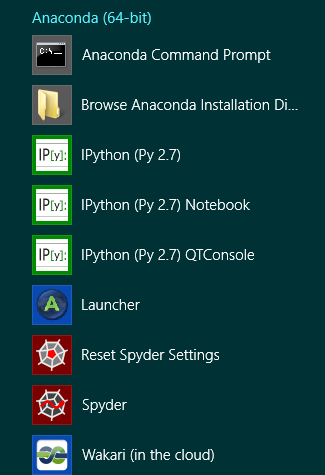
\includegraphics[scale=0.6]{Imagenes/ipython_notebook_01.png}
\caption{Accesos directos de Anaconda}
\end{wrapfigure}
%\begin{figure}[H]
%	\centering
%	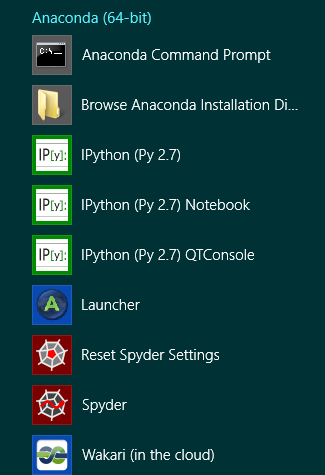
\includegraphics[scale=0.5]{Imagenes/ipython_notebook_01.png} 
%\end{figure}
Para quienes usen Windows, en la carpeta de programas encontrarán un ícono de acceso directo que debemos de elegir para abrir la sesión de \texttt{Ipython notebook}, revisen la siguiente imagen:
\\
\\
Esto generará cierta información sobre el servidor del notebook en la consola, y abrirá el navegador web\footnote{Es posible modificar en la configuración, el navegador de tu preferencia, en caso de que tuvieses varios instalados en tu equipo, pero elegirá el que tengas seleccionado por default.} a la dirección URL de la aplicación web (por defecto, http://127.0.0.1:8888). 
\\
\\
La página de inicio de la aplicación web notebook IPython muestra el tablero principal, así como los notebooks disponibles actualmente en el directorio (de forma predeterminada, el directorio desde el que se inició el servidor) 
\\
\\
\\
\\
\\
\\
Es posible crear nuevos notebook desde el tablero principal con el botón Nuevo Notebook, o abrir los ya existentes haciendo clic en su nombre. También puedes arrastrar y soltar archivos notebook \texttt{.ipynb} y archivos de código fuente de Python estándar \texttt{.py} en el área que muestra la lista de notebooks. 
\\
\\
Cuando se inicia un servidor de notebooks en la línea de comandos, también puedes abrir directamente un notebook en particular, sin pasar por el tablero principal, con \texttt{ mi\_notebook.ipynb notebook ipython}. La extensión \texttt{.ipynb} se asume por defecto si no se escribe la extensión.
\section{La interfaz de usuario del notebook.}
Cuando se crea un nuevo notebook, se presentará con el nombre del notebook, una barra de menús, una barra de herramientas y una celda de código vacío. 
\begin{figure}[H]
	\centering
	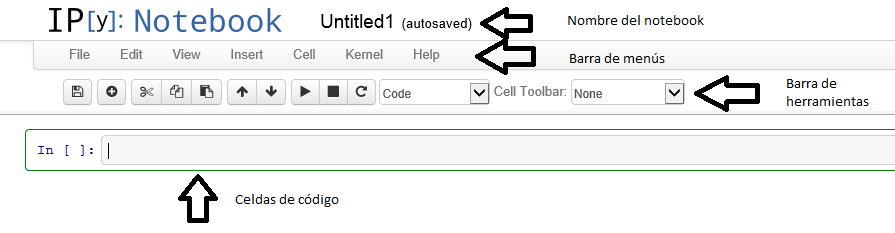
\includegraphics[scale=0.6]{Imagenes/ipython_notebook_04.png} 
\end{figure}
\textbf{Nombre del notebook}: El nombre del notebook se muestra en la parte superior de la página, junto al logo de  IP [y]:
\\
\\
Este nombre indica el nombre del notebook \texttt{.ipynb}. Al hacer clic sobre el nombre del mismo aparece un cuadro de diálogo que te permite cambiar el nombre, por lo tanto, el cambio de nombre de un cuaderno de ''Untitled0'' a ''Mi primer notebook'' en el navegador, cambia el nombre del archivo \texttt{Untitled0.ipynb} a  \texttt{Mi primer notebook.ipynb}.
\\
\\
\textbf{Barra de menú}: La barra de menú presenta diferentes opciones que se pueden usar para manipular la operación del notebook. 
\\
\\
\textbf{Barra de herramientas}: La barra de herramientas proporciona una forma rápida de realizar las operaciones más utilizadas dentro del notebook, haciendo clic en un ícono. 
\\
\\
\textbf{Celda de código}: Te permite editar y escribir nuevo código, con resaltado completo de sintaxis  y la implementación del tabulador. Por defecto, el idioma asociado a una celda de código es \python.
\section{Agregar un notebook a nuestro equipo.}
El manejo de los archivos \texttt{*.ipynb} para agregarlos a Ipython notebook es muy sencillo: basta que le indiquemos a nuestra aplicación en dónde se ubica el mismo, mediante una cuadro de diálogo:
\begin{figure}[H]
	\centering
	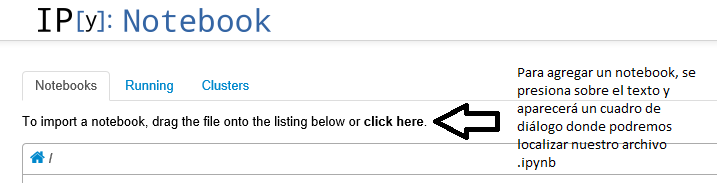
\includegraphics[scale=0.6]{Imagenes/ipython_notebook_08.png} 
\end{figure}
Es recomendable que dejen en una carpeta todos los archivos notebook \texttt{*.ipynb} que estaremos enviando durante el curso, con la finalidad de concentrar sus materiales.
\\
\\
Elegimos la ruta donde tengamos nuestro archivo y lo seleccionamos para la carga en el navegador web:
\begin{wrapfigure}{R}{5cm}
	\centering
	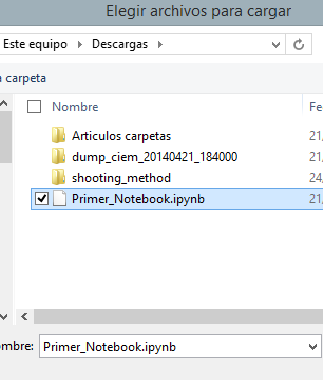
\includegraphics[scale=0.6]{Imagenes/ipython_notebook_06.png}
	\caption{El cuadro de diálogo permite ubicar nuestro archivo.}
\end{wrapfigure}
\newpage
Nota al margen: Hay que considerar que los archivos notebook \texttt{*.ipynb} no son precisamente como tal, archivos de código \texttt{*.py} los cuales podemos manejar y editar con Spyder o con otro editor de texto; los archivos notebook cuentan con un formato propio para ser reconocidos por la aplicación IPython notebook, si queremos abrir como tal el archivo, veremos que incluye otro tipo de información que al querer ejecutar desde la consola o con spyder, tendremos muchos errores de ejecución, debido a que el archivo como se lee, tiene la estructura de un archivo en lenguaje de marcado extensible (XML) que si bien incluye el código, tiene además, otras estructuras que el navegador requiere para ubicar lo que es la celda, marcar el color de la palabra, etc. Por ello es importante que la misma aplicación notebook, sea quien abra y ejecute el código contenido en el archivo.
\\
\\
El último paso que tenemos que realizar para contar con nuestro notebook en la lista del navegador, es presionar el botón azul de \emph{upload}, con ello, ya veremos en el listado todos aquellos cargados y listos para trabajar con ellos.
\begin{figure}[H]
	\centering
	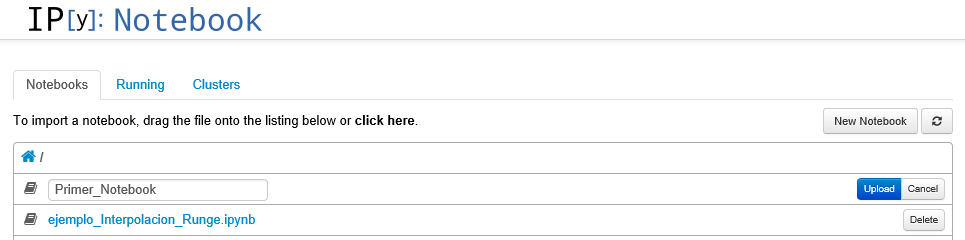
\includegraphics[scale=0.6]{Imagenes/ipython_notebook_05.png} 
\end{figure}
Y al dar click sobre el nombre del notebook ya en la lista, se abrirá el archivo para revisarlo y trabajar con él.
\begin{figure}[H]
	\centering
	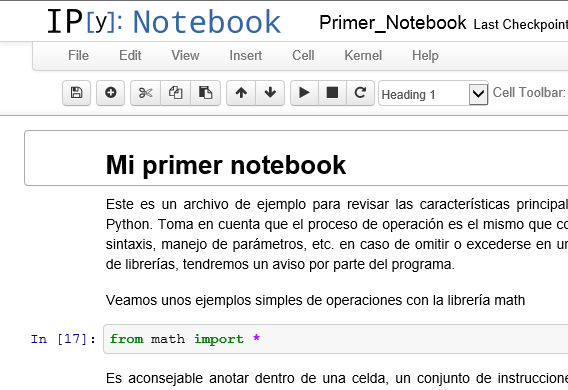
\includegraphics[scale=0.6]{Imagenes/ipython_notebook_07.png}
	\caption{El notebook ya listo para revisión.} 
\end{figure}
\section{Controles para la interfaz de usuario del notebook.}
Hay dos modos de operación para el manejo del notebook: Modo de edición y modo de comando.
\\
\\
\textbf{El modo de edición}: Se indica con un borde de la celda verde y el prompt se muestra en el área de edición: 
\begin{figure}[H]
	\centering
	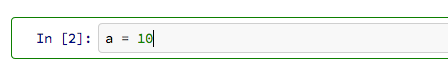
\includegraphics[scale=0.6]{Imagenes/ipython_notebook_09.png}
\end{figure}
Cuando una celda se encuentra en modo de edición, se puede escribir en la celda, como un editor de texto normal. Entramos en el modo de edición pulsando \texttt{Enter} o usando el ratón para hacer click en el área de edición de una celda. 
\\
\\
\textbf{El modo de comando:} Se indica mediante un borde de la celda gris: 
\begin{figure}[H]
	\centering
	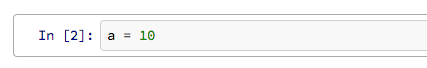
\includegraphics[scale=0.6]{Imagenes/ipython_notebook_10.png}
\end{figure}
Cuando se está en el modo de comandos, tenemos la capacidad de editar el notebook en su conjunto, pero no podemos escribir en celdas individuales. Lo más importante, en el modo de comando, se le asignas atajos al teclado que permiten realizar acciones sobre el notebook y celdas de manera eficiente. Por ejemplo, si se encuentra en modo de comando y pulsa \emph{c}, se copia la celda actual, sin necesidad de algún modificador. No tratas de escribir en una celda en modo de comando, puede ocurrir cualquier cosa inesperada.
\\
\\
Entra en el modo comando presionando la tecal \emph{Esc} o haciendo click fuera del área de editor de una celda. 
\\
\\
\textbf{Navegación con el ratón.} De la barra de herramientas que tenemos disponible en el notebook, el botón de \emph{play} nos permite ejecutar la celda en la que nos ubicamos, siendo el botón más relevante para la revisión de los archivos notebook.
\\
\\
Con el ratón podrás elegir la celda a partir de la cual, se inicia la ejecución del código, ya que celdas con texto, formalmente no ejecutan alguna acción, permiten la secuencia de revisión del texto explicativo, pero se recomienda que ejecutes cada celda desde el inicio, de esta manera, se podrá revisar y si la instrucción de código lo indica, cargaría una librería en particular y tenerla disponible durante la sesión.
\\
\\
Una manera alterna de ejecutar las celdas con el teclado, es mediante la combinación de \textbf{Shift} + \textbf{Enter}.
\section{Cerrar el notebook.}
Una vez que terminamos de revisar o editar un notebook, es importante cerrar el servicio web que se habilitó para visualizar y ejecutar el código.
\\
\\
Abrimos el menú File, luego el comando: Close and Halt, lo que cierra el notebook y cancela el servicio web, como estamos cerrando una página web, el navegador nos preguntará si queremos en realidad cerrar la página, lo que debemos de confirmar. Lo que nos resta es cerrar la terminal que se abre, para ello presionamos conjuntamente \textbf{Ctrl} + \textbf{C}, con lo que recuperamos el prompt de nuestra terminal.
\\
\\
Esta es una revisión express de la operación, uso y manejo de un notebook de IPython, no es lo único que deberían de trabajar, sino que les dejamos la carta abierta para que ustedes extiendan y exploten al máximo estas nuevas herramientas que están orientadas al aprendizaje. Para mayor información, pueden consultar la página del proyecto de IPython: \url{http://ipython.org/ipython-doc/stable/notebook/notebook.html}
\end{document}